%%%%%%%%%%%%%%%%%%%%%%%%%%%%%%%%%%%%%%%%%%%%%%%%
% 4: Diseño y resolución del trabajo realizado
%%%%%%%%%%%%%%%%%%%%%%%%%%%%%%%%%%%%%%%%%%%%%%%%
\chapter{Diseño y resolución del trabajo realizado}
\label{diseno}

Después de estudiar cual es la situación actual de la enseñanza de la programación a un nivel global y los diferentes proyectos que promueven el \emph{pensamiento computacional}, en éste capítulo se analizarán cuales son las necesidades del proyecto Robode y como se han resuelto.

Como ya se ha mencionado anteriormente, se ha creado el simulador de un robot, al que hemos denominado \emph{Robode}, que se integrará en la plataforma Descubre la programación. Robode se encuentra dentro de un mundo en el que puede moverse con libertad y con el que interactua. El robot posee dos ruedas que se mueven independientemente (con un motor para cada una de ellas) y dispone de sensores que informarán de posibles colisiones con obstáculos. También, el robot puede detectar color en el suelo debajo del mismo. Ésta capacidad se usará para detectar líneas pintadas de negro en el suelo.

Adicionalmente, el robot y el mundo en el que este se encuentra será dibujado en el elemento \emph{canvas} de HTML5, al igual que ocurre en la plataforma Descubre. El \emph{canvas} establece un \emph{lienzo} en el que se pueden dibujar gráficos\footnote{Los gráficos pueden ser en 2 o 3 dimensiones, pero en el simulador que se desarrollará solo se hará uso de gráficos 2D.}. De igual modo, HTML5 proporciona muchas funciones para dibujar en el \emph{canvas} de manera relativamente sencilla.


Como se puede ver, Robode es la unión de varios de los proyectos que se han analizado en el capítulo \ref{estado-arte}. Por una parte, la idea principal de crear un simulador es igual a la que se ha realizado en Robomind (el cual se analiza en la sección \ref{sec:robomind}) pero simulando un robot en un mundo continuo. El robot comparte características físicas con el robot Moway (analizado en la sección \ref{sec:moway}), como es la disposición de sensores (tanto externos como inferiores) y el funcionamiento y disposición de las ruedas. Por último, se ejecutará en un entorno web, como bien puede ser el ejemplo de las plataformas CodeHS (sección \ref{sec:CodeHS}) y Code.org (sección \ref{sec:Code.org}). 


En las secciones siguientes se va a estudiar como se ha diseñado y creado Robode, que características tiene y cual ha sido la implementación llevada a cabo. También se verá como se ha modificado la plataforma Descubre para integrar el simulador en ella. Pero antes, se analizará el nuevo modelo de programación que se ha creado y en el que se basa el simulador.



\section{Modelo de programación del simulador}
\label{sec:modelo-programacion}

El modelo de programación que presenta iJava actualmente consiste en crear una función principal \texttt{main} sin parámetros y que devuelve el tipo \texttt{void}. También, se puede usar la función \texttt{animate()}, tomando como argumento una función y ejecutándola en bucle. El resto es similar a un lenguaje imperativo. Un programa de ejemplo en iJava se puede encontrar en el código \ref{code:circulos-color-raton}.

El modelo de programación que se plantea para usar el simulador no es muy diferente. Para definirlo, se han estudiado los lenguajes de programación que usan Moway, Turtle, Scratch y Arduino y que ya se han mencionado anteriormente en este documento.


Primeramente se tiene una función principal, que se llamara \texttt{setup()} y que no recibirá parámetros y devuelve el tipo \texttt{void}. Esta función cumple el mismo papel que la función \texttt{main()} de iJava, pero se ha cambiado el nombrado para adecuarlo al estándar de Arduino y darle el significado de establecer los parámetros del robot y su comportamiento inicial. 

Por ejemplo, en la función \texttt{setup()} se podría programar el robot de manera que cuando inicia el programa, éste gire 180º y el programa termine. En \texttt{setup()} se puede programar un comportamiento estándar del robot. Pero también es necesario permitir que el robot reaccione al entorno y a posibles cambios que en este se producen. Por tanto, es necesario añadir otro elemento al modelo.

La función \texttt{loop()} ejecutará en bucle todas las instrucciones que en ella se encuentren. De esta manera, se permite una ejecución infinita que permita reaccionar a cambios del entorno. Esto se hará con la información que le llegue al robot a través de los sensores. 


No es necesario indicar que la función \texttt{loop()} se ejecute en bucle, a diferencia de iJava. En iJava se usaba la función \texttt{animate} que recibe una función como argumento y esta es ejecutada en bucle. La función \texttt{loop()} se comportará automáticamente de esta manera. En realidad, lo que hará el motor de iJava será llamar a la función \texttt{loop()} usando \texttt{animate(loop)} de manera transparente al programador. Esto ocurre solo si la función \texttt{loop()} ha sido definida en el código iJava.


En cuanto a la funcionalidad que ofrece la API del simulador para poder controlar al robot, se busca que las funciones ofrecidas sean lo más básicas posibles. La intención es que el programador tenga los elementos básicos y suficientes para manejar el robot. Si éste quisiera funciones más complejas, tendría que programarlas él mismo, contribuyendo así a su aprendizaje. 

A continuación vamos a listar todas las funciones que ofrece la librería del robot. Ademas, la API también ofrece un conjunto de variables de tipo \texttt{boolean} que permitirán conocer si los sensores están detectando colisiones o no.

\begin{itemize}
	\item \texttt{initRobot()}: Inicia, muestra y coloca el robot en su posición inicial.
	\item \texttt{power(potenciaIzq, potenciaDer)}: Establece la potencia con la que se moverá cada rueda. El primer argumento es para la rueda izquierda mientras que el segundo para la derecha. El valor de potencia estará entre 40 y -40. Un valor positivo moverá la rueda en dirección frontal y un valor negativo, posterior. Un valor de 0 hará que esa rueda deje de ejercer fuerza.
	\item \texttt{stop()}: Detiene el robot.
	\item \texttt{left()}: Gira el robot 90º en dirección contraria al sentido de las agujas del reloj.
	\item \texttt{wait(n\_milisegundos)}: Crea una espera de tiempo igual al número de milisegundos que se le pasan como argumento a la función. 
	\item \texttt{sensorNW}: Sensor de colisiones en la posición Noroeste. Un valor de \texttt{true} indica que está detectando colisiones.
	\item \texttt{sensorNE}: Sensor de colisiones en la posición Noreste. Un valor de \texttt{true} indica que está detectando colisiones.
	\item \texttt{sensorSW}: Sensor de colisiones en la posición Suroeste. Un valor de \texttt{true} indica que está detectando colisiones.
	\item \texttt{sensorSE}: Sensor de colisiones en la posición Sureste. Un valor de \texttt{true} indica que está detectando colisiones.
	\item \texttt{collisioning}: Devuelve \texttt{true} si alguno de los sensores anteriores está detectando una colisión.
	\item \texttt{sensorLL}: Sensor inferior izquierdo que detectará si Robode está sobre una línea.
	\item \texttt{sensorLR}: Sensor inferior derecho que detectará si Robode está sobre una línea.
\end{itemize}

Como se puede ver, se ofrecen diferentes variables de tipo \texttt{boolean} para saber si el robot está detectando con alguno de los sensores una colisión o si está sobre una línea. Por otra parte, se ofrece la función \texttt{wait()} que produce una espera de tiempo\footnote{En la sección \ref{animando-robode} se explica en detalle como se ha conseguido este efecto en el sistema \emph{monohilo} que implementa Javascript.} en la que no se ejecutarán nuevas instrucciones.

Un ejemplo que muestra el nuevo modelo de programación se puede ver en el código \ref{code:nuevo-modelo}.

\begin{lstlisting}[language={Java},label={code:nuevo-modelo}, caption={Programa de ejemplo que mueve al robot con el nuevo Modelo de programación establecido para el simulador.}]
int delay;
int potenciaDer;
int potenciaIzq;
void setup(){
	delay = 1000; // 1 segundo en milisegundos
	potenciaDer = 10;
	potenciaIzq = 10;
	//iniciamos el robot
	initRobot();
}

void loop(){
	//movimiento de las ruedas
	power(potenciaIzq, potenciaDer); 
	// esperamos 
	wait(delay);
	// detenemos el robot
	power(0, 0);
	//esperamos el doble de tiempo
	wait(delay * 2);
}
\end{lstlisting}

Los pasos descritos del funcionamiento del programa se enumeran a continuación:

\begin{enumerate}
	\item Se declaran las variables \texttt{delay}, \texttt{potenciaDer} y \texttt{potenciaIzq}. 
	\item Se ejecuta la función \texttt{setup()}:
\begin{itemize}
	\item Se establecen los valores de las variables \texttt{delay}, \texttt{potenciaDer} y \texttt{potenciaIzq}. 
	\item Se inicia el robot. Esto solo creará el robot en la posición inicial. 
\end{itemize}
	\item Se ejecuta la función \texttt{loop()}:
\begin{itemize}
	\item Se establece la potencia de las rueda derecha a \texttt{potenciaDer} y de la rueda izquierda a \texttt{potenciaIzq}.
	\item Se produce una espera de cantidad \texttt{delay} (1 segundo) en el que no se admiten nuevas instrucciones.
	\item Se establece la potencia de las rueda derecha a 0 y de la rueda izquierda a 0.
	\item Se produce una espera de 2 segundos en el que no se admiten nuevas instrucciones.
\end{itemize}
	\item Se repite el paso 3.
\end{enumerate}

Con respecto a función \texttt{loop()}, puesto que ya existe un bucle infinito en el programa, no es una buena práctica crear bucles infinitos\footnote{Obviamente, no hay ningún problema en definir bucles que recorran variables o realicen cálculos, por ejemplo.} en el simulador.

Por ejemplo, la forma de reaccionar a las colisiones sería la que se muestra en el código \ref{code:ejemplo-colisiones-robode}. En lugar de utilizar un bucle \emph{while} que espere hasta que se produzca una colisión, se comprueban con condiciones \texttt{if} o \texttt{if-else}.

\begin{lstlisting}[language={Java},label={code:ejemplo-colisiones-robode}, caption={Ejemplo de buenas prácticas en el uso de la API del simulador.}]
void setup() {
    initRobot();
}

void loop() {
	//por defecto, hacia delante
    power(10, 10);
	// Si colision delante, retrocedo hacia la izquierda
    if (sensorNW || sensorNE) {
        power(-10, -20);
    }
  	//si colision detras avanzo torciendo
    if (sensorSW) {
        power(20, 10);
    }
    
    if (sensorSE) {
        power(10, 20);
    }
}
\end{lstlisting}

Recapitulando, tenemos una función principal \texttt{setup()} que puede ser complementada con la función \texttt{loop()}, la cual ejecutará en bucle infinito que permitirá reaccionar al entorno según pasa el tiempo.

En la sección siguiente se estudiará como se ha modificado iJava para implementar este nuevo modelo de programación.

\subsection{Modificación del lenguaje iJava}
\label{sec:modificacion-ijava}

Para poder conseguir lo que se ha descrito anteriormente, es imprescindible realizar ciertos cambios en el compilador de iJava para que reconozca y ejecute las nuevas funciones de la API del robot.

Principalmente, el compilador de iJava consta de tres partes: el analizador sintáctico, el analizador semántico y el \emph{sandbox}. El \texttt{sandbox} contiene la implementación de las funciones de librería descritas en el analizador sintáctico. Éste ejecuta (en un entorno seguro) el código Javascript que se genera a partir del código fuente en iJava. Siempre y cuando todo el proceso de compilación se haya realizado con éxito. 

Para que las funciones de la API sean parte del lenguaje y se ejecuten como una más de iJava, hay que realizar tres grandes cambios. Estos son: (a) modificar el analizador semántico para cambiar la función principal \texttt{main} por \texttt{setup}; (b) añadir la definición de las funciones al analizados sintáctico y (c) añadir la implementación de las funciones al \emph{sandbox}.

Para el cambio (a), hay que modificar el analizador semántico de iJava (clase \texttt{iJavaSemantic}). El analizador semántico busca si la función \texttt{setup} (antes \texttt{main}) se ha definido y, si no la encuentra, devolverá un error que se mostrará por pantalla. Además, en el código Javascript que se genera como ejecución del programa del usuario (función \texttt{eval()}), se ha definido que la función \texttt{loop()} se ejecute en un bucle infinito siempre y cuando ésta se haya definido en el programa del usuario.

Para añadir las definiciones de nuevas funciones (cambio (b) ), hay que añadir al analizador sintáctico (clase \texttt{iJavaParser}) la definición de dichas funciones. También hay que indicar el número y tipo de parámetros de las funciones. Para el caso de las variables de los sensores, también hay que añadirlas como variables del sistema (de iJava) de tipo \texttt{boolean}.

Por último, el cambio (c) se consigue implementando las funciones de la API en el sandbox de iJava (clase \texttt{iJavaSandbox}). Las funciones y variables tienen que tener el mismo nombre, tipo y argumentos que las definidas en el analizador sintáctico para que el compilador las detecte y se puedan ejecutar.

En el apéndice \ref{anexo:ampliacion-ijava-API} se incluye las secciones más importantes del código que implica los cambios arriba mencionados.


Adicionalmente a estos cambios, también se han eliminado las funciones de librería de gráficos y de entrada estándar (teclado y ratón) puesto que no aportaban interés a la programación con un robot. 


\section{Integración en Descubre del simulador}
\label{sec:integracion-descubre}


Descubre la programación\cite{descubre} es una plataforma online que se enfoca en enseñar a programar a alumnos de Educación Primaria y Secundaria. Para ello, se provee de un entorno que permite programar en iJava\cite{sanchez2009ijava} y compilar el código ejecutado. La salida se muestra por una pantalla dispuesta para ello.

Esto se realiza gracias al compilador que implementa Descubre. Dicho compilador obtendrá el código escrito en iJava y lo analizará en busca de errores. Si el análisis sintáctico y semántico no encuentra ningún problema, entonces realizará una traducción de iJava a Javascript para ejecutar dicho código en el navegador. La salida se mostrará por el elemento \texttt{canvas} de HTML5.

Para explicar como está creada la plataforma Descubre, se muestra el diagrama de clases de Descubre en la figura \ref{fig:diagram-ijava}. La clase principal de Descubre es \texttt{(index)}, que representará al fichero HTML principal.

\begin{figure}[!ht]
	\begin{centering}
		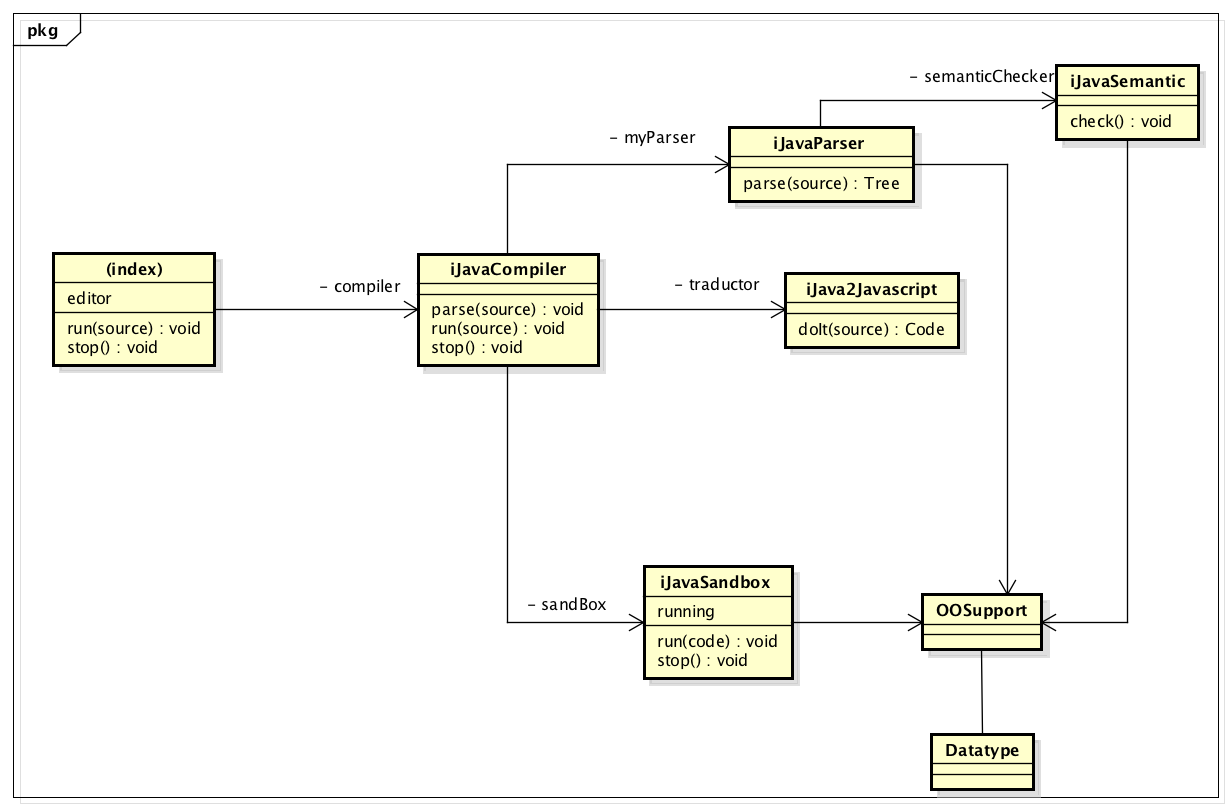
\includegraphics[width=1\textwidth]{images/diagram-ijava.png}
			\caption{Diagrama de clases de la plataforma Descubre: punto de partida.}
				\label{fig:diagram-ijava}
	\end{centering}
\end{figure}

Para entender como se relacionan todas estas clases y cual es la comunicación entre ellas, en la figura \ref{fig:comunication-ijava} se puede ver un diagrama de comunicación simple que se produciría cuando un usuario hace click en el botón \texttt{run} de Descubre.

\begin{figure}[!ht]
	\begin{centering}
		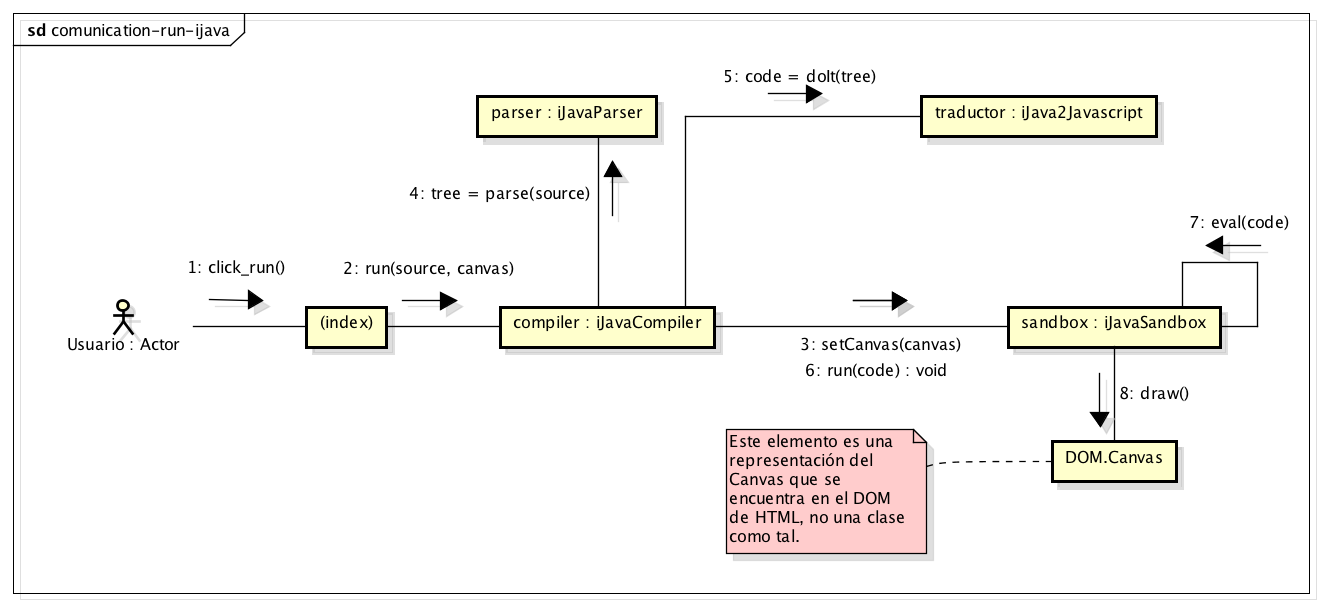
\includegraphics[width=1\textwidth]{images/comunication-run-ijava.png}
			\caption{Diagrama de comunicación de la función \texttt{run()}.}
				\label{fig:comunication-ijava}
	\end{centering}
\end{figure}

En resumen, el diagrama de comunicación muestra cuales son los pasos que se llevan a cabo para ejecutar un código escrito en Javascript. También hay que tener en cuenta que el \emph{canvas} no es una clase al uso. Aún así, se ha decidido incluirlo de esta manera para poder representar quién realiza la acción de pintar (método \texttt{draw()}). Esto cambiará cuando entre en juego el simulador.

Es la clase \texttt{iJavaSandbox} la que ejecuta el código convertido a Javascript con la función \texttt{eval()} de Javascript. En esta clase estará la implementación de todas las funciones de librería que ofrece iJava en el lenguaje: funciones matemáticas, funciones para pintar el \emph{canvas}, entrada y salida, etc.

En las secciones siguientes se analizará que cambios se han realizado para integrar el simulador del robot en Descubre.

\subsection{Modificación de la plataforma Descubre}
\label{sec:modificacion-descubre}


En la sección \ref{sec:modificacion-ijava} se ha hablado de los pasos necesarios para modificar el compilador de iJava para añadir nuevas librerías. Pero para añadir el simulador, es necesario añadir toda la lógica de la simulación al compilador. El control del robot y del mundo se implementa en la clase \texttt{Robode}.

La clase \texttt{Robode} recibirá los mensajes del \emph{Sandbox} que le dirá como tiene que mover el robot (potencia de las ruedas, detenerse por completo, etc) y, a la misma vez, \texttt{Robode} le comunicará al \emph{Sandbox} cuando un sensor está detectando colisiones. La clase\texttt{Simulator} encapsula detalles de la simulación, como puede ser la configuración inicial del robot (posición, tamaño, etc) o del mundo (ancho, alto, etc). 

Además, se han representado elementos básicos del motor físico que se ha utilizado para la simulación. Esto es importante ya que otorga una visión general del funcionamiento del motor físico y su relación con el simulador y Robode. Ésto último será útil cuando se vea el uso e implementación del motor físico en la sección \ref{sec:motor-fisico}.

En la figura \ref{fig:diagram-ijava-robode} se puede ver el nuevo diagrama de clases con la inserción del simulador a iJava. También, en la figura \ref{fig:comunication-run-robode}, se pueden ver los pasos que se producirían al ejecutar un código iJava que ejecuta funciones del robot. 

Como se puede ver, el  \emph{Sandbox} envía dos mensajes diferentes para comunicarse con \texttt{Robode} indicando el \emph{canvas} y que tiene que ejecutar cierta orden. Ahora, es la clase \texttt{Robode} la que dibujará en el \texttt{canvas} y no el \emph{Sandbox}. La razón de esto se explica más adelante, en la sección \ref{animando-robode}.

\begin{figure}[!ht]
	\begin{centering}
		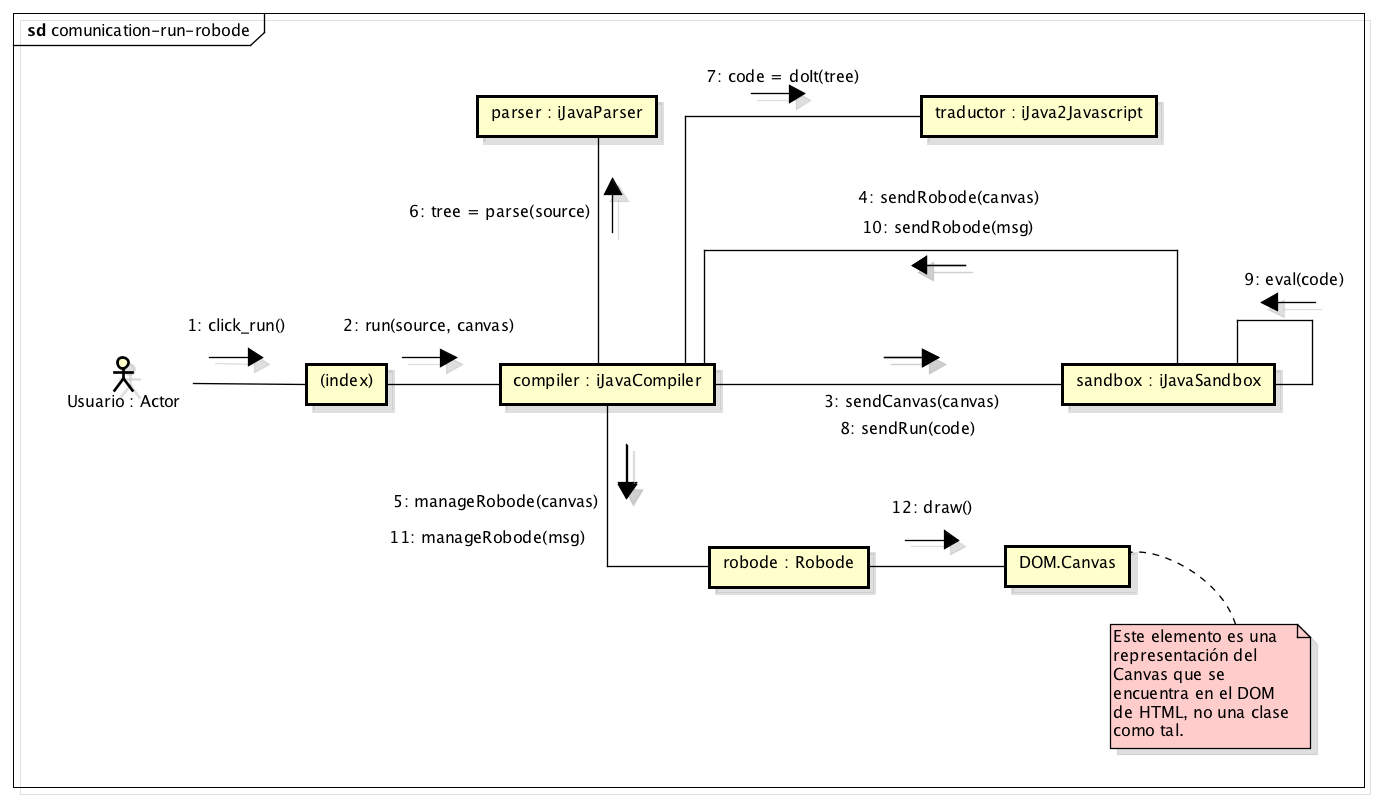
\includegraphics[width=0.8\textwidth]{images/comunication-run-robode.png}
			\caption{Diagrama de comunicación que se produce cuando se ejecuta un código Java después de integral el simulador con Descubre.}
				\label{fig:comunication-run-robode}
	\end{centering}
\end{figure}

\begin{figure}[!ht]
	\begin{centering}
		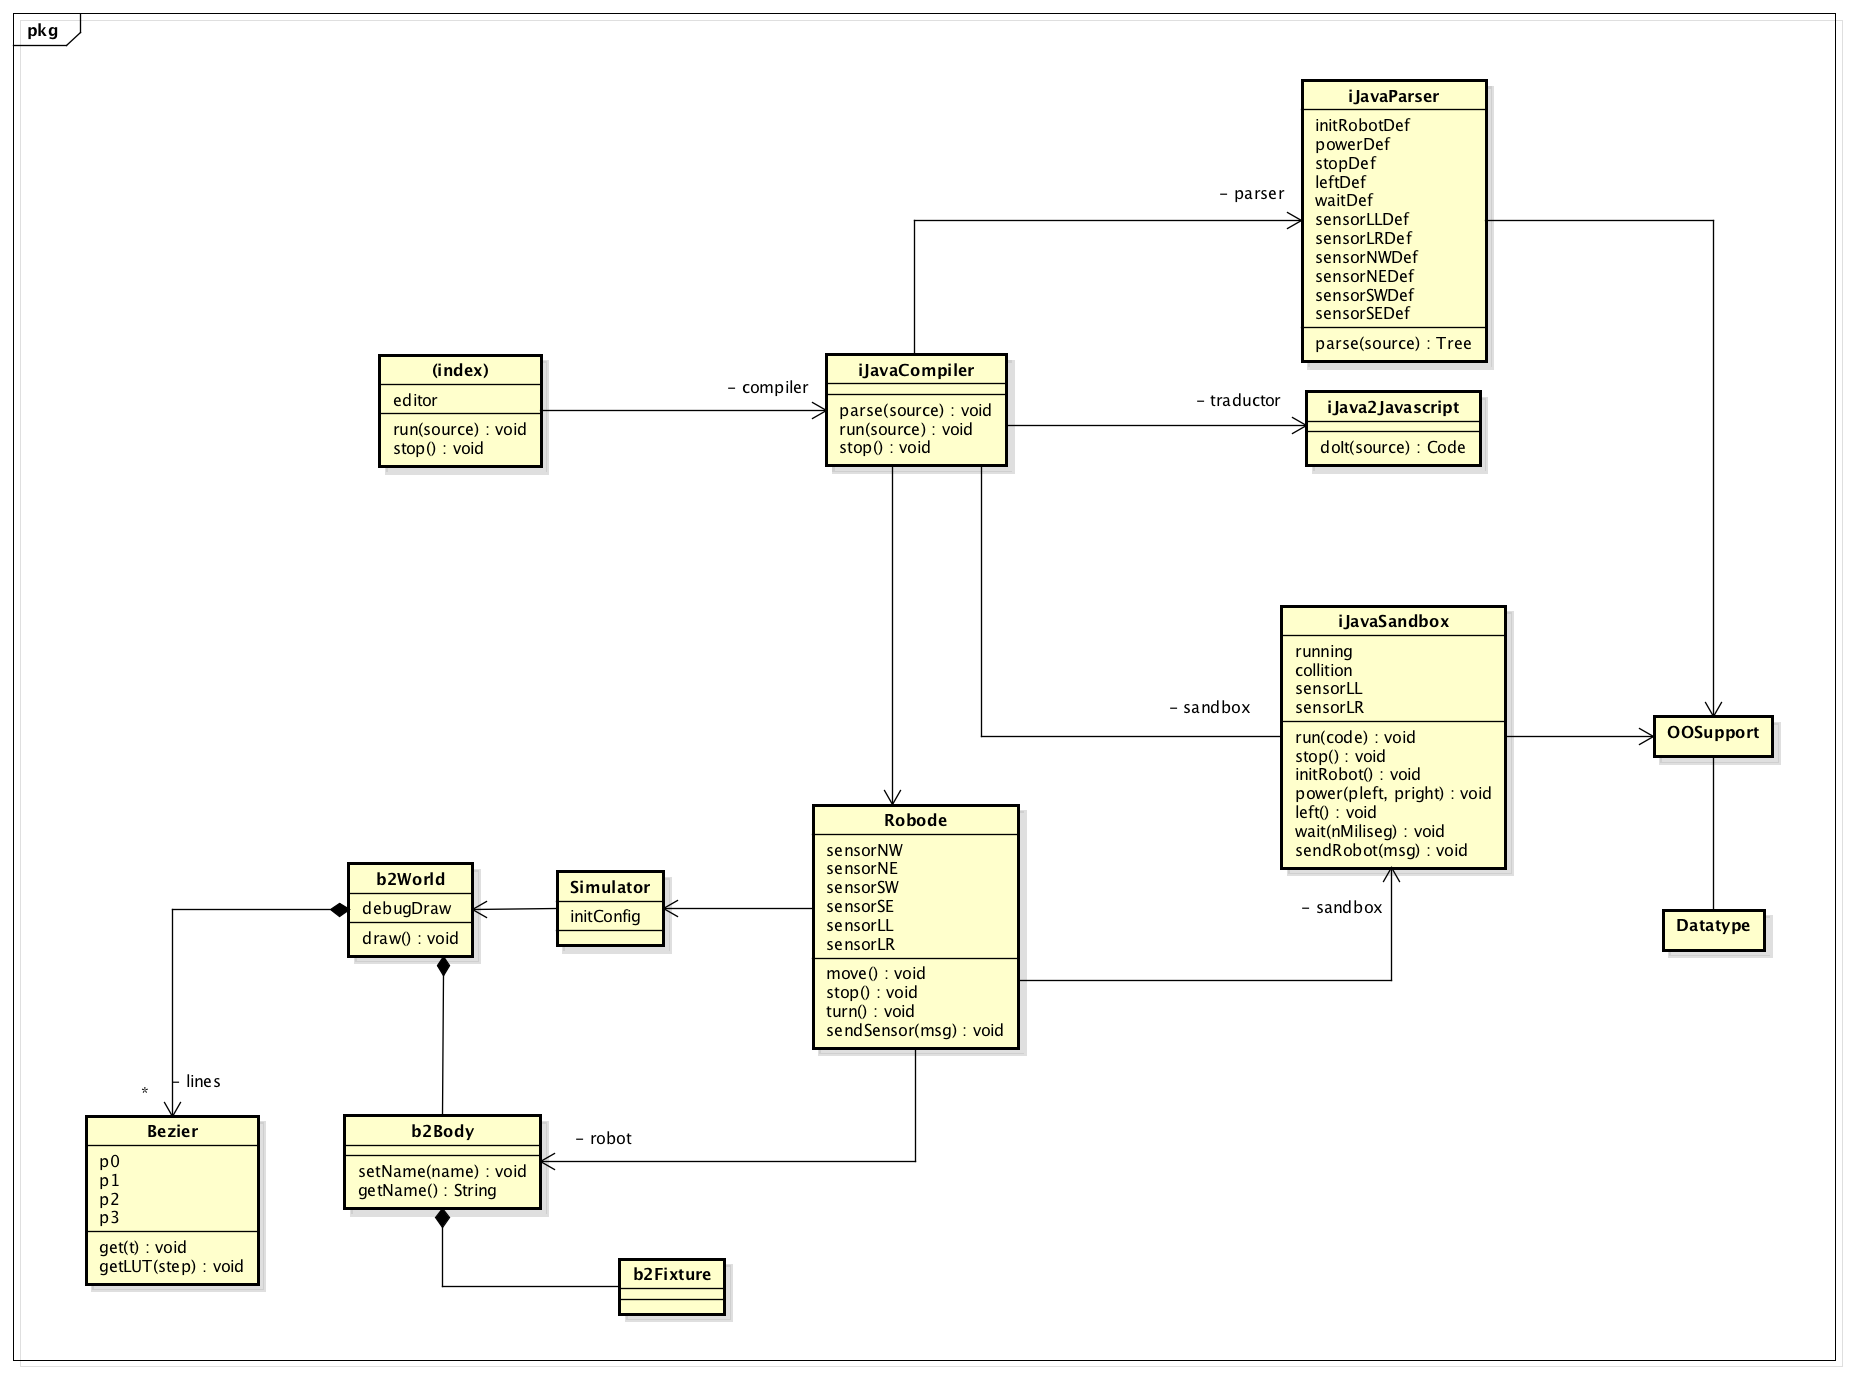
\includegraphics[width=1.2\textwidth]{images/diagram-ijava-robode.png}
			\caption{Diagrama de clases de la aplicación después de integrar el simulador con Descubre.}
				\label{fig:diagram-ijava-robode}
	\end{centering}
\end{figure}




\section{Motor físico}
\label{sec:motor-fisico}

El simulador representa un mundo con un robot y una serie de obstáculos que interfieren entre ellos. Los obstáculos pueden colisionar entre ellos o con el robot. También es necesario simular líneas en el suelo y la detección de las mismas. Todo ello con un paso del tiempo realista. Para ello, se necesita utilizar un motor físico que simule la creación de cuerpos en el mundo, su movimiento por el mismo y el contacto entre ellos, generando una reacción similar a la producida en el mundo real.

Para la creación del mundo y de las físicas que gestionan las colisiones y la interacción entre todos los elementos del simulador se han estudiado dos motores físicos: PhysicsJS\footnote{Página oficial de la librería PhysicsJS (\url{http://wellcaffeinated.net/PhysicsJS}).} y Box2D\footnote{El manual de uso de Box2D se puede encontrar en \cite{box2d-manual}. La documentación del proyecto se puede encontrar en (\url{http://www.box2dflash.org/docs/2.1a/reference/}).} \cite{box2d}. Dos librerías muy versátiles y de software libre que trabajan sobre entornos web.

PhysicsJS  es una librería escrita enteramente en Javascript por Jasper Palfree que aún está en fase beta. Por otra parte, Box2D es una famosa librería implementada originalmente para Flash\footnote{Página oficial de la librería Box2D para Flash (\url{http://www.box2dflash.org}).} con una gran comunidad de programadores utilizando dicha librería, lo cual siempre es de ayuda para resolver dudas y solucionar problemas. 

Box2D ha sido portada a Javascript dos veces. Una de ellas por Yayushi Ando y se llama Box2Djs\footnote{Página oficial de Box2Djs (\url{http://box2d-js.sourceforge.net}).} pero el proyecto no ha sido continuado y está desactualizado. El otro intento de llevar Box2D a Javascript ha culminado en Box2Dweb\footnote{El repositorio de Box2Dweb está alojado en GitHub (\url{https://github.com/hecht-software/box2dweb}).}. Como se puede leer en \cite[capítulo 13]{box2d-manual}, Box2D usa una serie de aproximaciones para representar las colisiones de manera eficiente. Principalmente, son dos las limitaciones que podría afectar al simulador del robot: (a) existe un desliz de aproximadamente 0.5 cm entre la forma que tiene un cuerpo y la colisión del mismo y (b) Box2D no maneja correctamente los cuerpos cóncavos. 

Al final, se ha establecido que la librería a utilizar será Box2Dweb. En cuanto a las limitaciones que puedan afectar a Robode, estas no son un gran problema a la solución del simulador puesto que: el desliz producido en limitación (a) es muy pequeño y en el caso del simulador, impercetible. Con respecto a la limitación (b), en el caso de que se quiera construir cuerpos cóncavos, se puede solucionar creando más de un cuerpo convexo que cree una forma \emph{global} cóncava.

Una vez que se ha aclarado que la librería utilizada es \texttt{Box2Dweb}, por simplicidad, a partir de ahora nos referiremos a ésta simplemente como \texttt{Box2D}.

\subsection{Definición del Mundo}
\label{sec:definicion-mundo}

En \texttt{Box2D} existen una serie de objetos que representan al mundo y los diferentes elementos que lo componen.  Estos son: el Mundo (World), los Cuerpos (Bodies), los Accesorios (Fixtures) y las Articulaciones o elementos constrictores (Joints).

El núcleo de Box2D es el objeto \emph{World}, el cual define los parámetros básicos que regirán la simulación más tarde. Estos parámetros pueden ser el ratio de actualización o la gravedad. También crea y almacena el resto de objetos de Box2D, como los \emph{Bodies}, las \emph{Fixtures} y los \emph{Joints}, entre otros.

Para la creación de nuestro mundo, se ha decidido que tendrá una vista \emph{top-down}, es decir, una vista del mundo desde arriba, desde el cielo. De esta manera se consigue una vista superior de todo el circuito simplificando la comprensión del movimiento del robot sobre el circuito.

Una de las características más importantes de \texttt{Box2D} es la posibilidad de dotar a la aplicación que se está creando de un efecto gravitatorio de manera nativa al motor. Lo normal sería establecer éste valor con un vector de dirección hacia el suelo (hacia la parte baja de la pantalla) con la fuerza que se quiera simular. Esto provocaría que los cuerpos del mundo estuvieran constantemente sometidos a una fuerza que los mueve en dirección a ese vector, normalmente hacia el suelo.  

En el caso de Robode, al tener una vista superior del circuito, establecer una gravedad provocaría que el robot y el resto de cuerpos del circuito se movieran de forma anómala. Por esto, es necesario crear un mundo sin gravedad. En el listado del código \ref{code:world-gravedad} podemos ver como se ha establecido la gravedad del mundo a un vector con valor 0 en ambos ejes de coordenadas. 

\begin{lstlisting}[language={Javascript},label={code:world-gravedad}, caption={Definición del objeto \texttt{World} en Box2D con gravedad 0 y permitiendo que los cuerpos sean capaces de dormir.}]
Simulator.World = new b2World(
	new b2Vec2(0, 0), //gravity
	true //allow sleep
);
\end{lstlisting}

Otra característica importante en Box2D y que tiene un gran impacto en el rendimiento de la simulación es que los cuerpos puedan \emph{dormir}. Un cuerpo \emph{dormirá} cuando éste esté inactivo, es decir, cuando no esté siendo sometido a ninguna fuerza o sobre el se aplican fuerzas, pero éstas no son capaces de alterar su estado (posición, ángulo de giro, etc)\footnote{Esto ocurre generalmente cuando un objeto está sobre una superficie cuya forma y la del cuerpo hace que éste se mantenga quieto. Un ejemplo de esto puede ser un cuadrado sobre una superficie plana y horizontal con una gravedad hacia el suelo.}. En la línea 3 del listado de códigos \ref{code:world-gravedad} se puede ver como se ha establecido que los cuerpos del mundo sean capaces de dormir. Así, se consigue que el motor no simule los cuerpos que estén inactivos, mejorando el rendimiento de la aplicación.

Por último, queda definir el \emph{paso del tiempo} en Box2D. Para ello, es necesario ejecutar la función \texttt{Simulator.World.Step()} cada vez que queramos que se ejecute un \emph{paso} en nuestro mundo (esto es equivalente a un \emph{tic} de reloj). Esta función ordenará al motor que aplique todas las fuerzas necesarias sobre los cuerpos del mundo (gravedad, colisiones, deslizamientos, etc). Obviamente, es en este momento cuando se ejecutará la detección de colisiones por parte del motor de físicas. Justo después de ejecutar un paso se deben eliminar las fuerzas que afectan a los objetos para que se produzca un movimiento y efecto natural de las distintas fuerzas en los cuerpos. Esto se consigue con la función \texttt{Simulator.World.ClearForces()}.

En la figura \ref{fig:step-box2d} se muestra una representación de lo que ocurre en el motor de Box2D cada vez que se ejecuta un \emph{step}. En el código \ref{code:world-step} se puede ver con más detalle las funciones básicas que se deben ejecutar para que se produzca una actualización del mundo en Box2D.


\begin{lstlisting}[language={Javascript},label={code:world-step}, caption={Actualización del mundo en \texttt{Box2D}.}]
// (...)
Simulator.World.Step(
	1 / 60, //frame-rate
	10, //velocity iterations
	10 //position iterations
);

Simulator.World.ClearForces();

// (...)
\end{lstlisting}

En el apéndice \ref{anexo:creacion-elementos-box2d} se analizará en detalle las características básicas y más importantes de los objetos \texttt{Body}, \texttt{Fixture} y \texttt{Joint} de Box2D para entender como se crean elementos en Box2D. Por último, en la sección siguiente se explicará como se ha construido el robot y sus diferentes partes.


\begin{figure}[!ht]
	\begin{centering}
		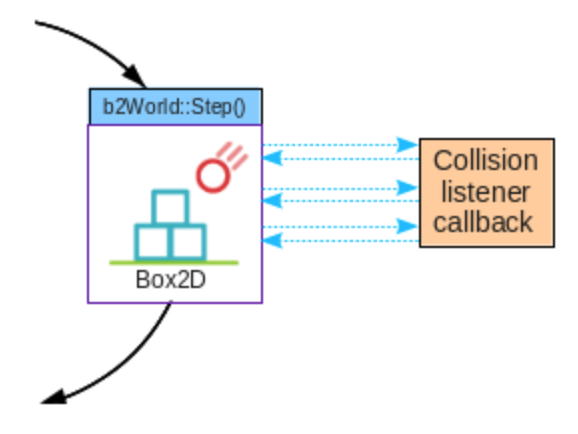
\includegraphics[width=0.5\textwidth]{images/step-box2d.png}
			\caption{Representación de lo que ocurre cada vez que se realiza la llamada a la función \texttt{Step()} en Box2D. Obtenido de \cite{box2d}.}
				\label{fig:step-box2d}
	\end{centering}
\end{figure}


\subsection{Construcción del robot}
\label{sec:contruccion-robot}

Para la creación del robot, un referente importante ha sido el robot Moway. La forma y disposición de los sensores es similar a la simulada en Robode. Otro objetivo a cumplir era el de crear una simulación que imitara un comportamiento natural del robot a la hora de moverse, de chocar o de detenerse. Por tanto, se han establecido diferentes propiedades en los cuerpos para cumplir este objetivo.

Anteriormente ya se ha mencionado que el robot tendrá 2 ruedas, 2 sensores inferiores (que se usaran para detectar líneas) y otros 4 que detectan colisiones. Todos estos elementos del robot están modelados en cuerpos separados. No obstante, será necesario que se mantengan unidos y se muevan a la vez. En la figura \ref{fig:robot-skel} se puede ver un esqueleto del robot con las partes diferenciadas y los elementos que unen a las diferentes partes (en azul).

La creación de cada una de las partes se explicará en las secciones siguientes.

\begin{figure}[!ht]
	\begin{centering}
		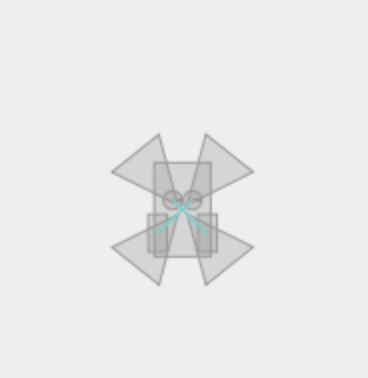
\includegraphics[width=0.5\textwidth]{images/robot-skel.png}
			\caption{Esqueleto del robot que muestra los diferentes \emph{bodies} y \emph{joints} que lo forman.}
				\label{fig:robot-skel}
	\end{centering}
\end{figure}


\subsubsection*{Cuerpo principal}
\label{sec:cuerpo-principal}

El cuerpo principal está modelado como un rectángulo. Éste será más largo que ancho y tendrá el resto de cuerpos (sensores y ruedas) \emph{atados} a él con \emph{joints}. El cuerpo principal de Robode será dinámico, así como los sensores y ruedas.

La forma se ha creado usando una fixture con forma poligonal. Se ha utilizado la función \texttt{SetAsBox()} que permite definir el ancho y alto del polígono, creándolo con forma rectangular. El ancho del robot será de 6 píxeles mientras que su largo medirá 10 píxeles.

En el listado de código \ref{code:creacion-cuerpo-principal} se puede ver el código que construye el cuerpo principal de Robode.

\begin{lstlisting}[language={Javascript},label={code:creacion-cuerpo-principal}, caption={Creación del cuerpo principal del robot utilizando la librería Box2dweb.}]
// Body definition
var bodyDef = new b2BodyDef(); 
bodyDef.type = b2Body.b2_dynamicBody;
bodyDef.position.Set(posX, posY);
bodyDef.linearDamping = 8;
bodyDef.angularDamping = 8;

// Fixture definition
var fixDef = new b2FixtureDef(); 
fixDef.density = 40;
fixDef.friction = 1;
fixDef.restitution = 0;
// Polygon Shape as a box
fixDef.shape = new b2PolygonShape(); 
fixDef.shape.SetAsBox(width, height);

// Create BODY robot
var robot = Simulator.World.CreateBody(bodyDef);
robot.setName("robot");

// Add fixture to body
robot.CreateFixture(fixDef);
\end{lstlisting}


\subsubsection*{Ruedas}

Las ruedas de Robode se simularan con dos polígonos con forma rectangular (método \texttt{SetAsBox()} de la clase \texttt{b2PolygonShape}). Su posición está retrasada con respecto al centro del cuerpo principal y su ancho es de 2 píxeles mientras que su alto mide 4 píxeles. En el listado de código \ref{code:creation-wheel} se puede ver como se han construido las ruedas. También se han mantenido los valores de densidad, fricción y restitución del cuerpo principal, reduciendo así la posibilidad de comportamientos anómalos durante una colisión.

\begin{lstlisting}[language={Javascript},label={code:creation-wheel}, caption={Función que crea las ruedas de Robode.}]
function createWheel(x, y) {

	var bodyDef = new b2BodyDef();
	bodyDef.type = b2Body.b2_dynamicBody;
	bodyDef.position.Set(x, y);
	
	var fixDef = new b2FixtureDef();
	fixDef.density = 40;
	fixDef.friction = 1;
	fixDef.restitution = 0;
	fixDef.isSensor = false;

	fixDef.shape = new b2PolygonShape();
	fixDef.shape.SetAsBox(0.2, 0.4);
	
	var wheelBody = Simulator.World.CreateBody(bodyDef);
	wheelBody.setName("wheel");
	wheelBody.CreateFixture(fixDef);
	return wheelBody;
}
\end{lstlisting}

Además, se creará un \emph{joint} que mantendrá unidas las ruedas con el cuerpo principal de Robode. En el listado de código  \ref{code:wheel-joint} se puede ver la creación del joint que une el coche con la rueda.

\begin{lstlisting}[language={Javascript},label={code:wheel-joint}, caption={Función que crea el joint que une la rueda al coche.}]
function addWheelJoint(mybody, mywheel) {

	var revoluteJointDef = new b2RevoluteJointDef();
	revoluteJointDef.Initialize(mybody, mywheel, mywheel.GetWorldCenter());

	revoluteJointDef.enableMotor = true;
	revoluteJointDef.motorSpeed = 0;
	revoluteJointDef.maxMotorTorque = Number.MAX_SAFE_INTEGER;
	revoluteJointDef.enableLimit = true;

	return Simulator.World.CreateJoint(revoluteJointDef);
}
\end{lstlisting}

La función \texttt{Initialize()} recibe como parámetros los dos cuerpos que van a ser unidos por el joint y el punto en el que se realizará el ancla (para eso se utilizará la función \texttt{GetWorldCenter()} de la clase \texttt{Body} para obtener el punto del mundo en el que se encuentra un cuerpo).

Se activará la propiedad de motor en las ruedas y se le dará un valor inicial de 0. También se establecerá el valor máximo de torsión del joint para evitar que ante una fuerza de giro muy grande, el joint se mueva de su sitio. Por último, se activará un límite para que las ruedas no se muevan de su sitio ya que es esta propiedad la que define si el ancla será fija o permitirá movimiento con respecto a la separación de los dos cuerpos.

El movimiento del robot se simulará con el movimiento que se producirá en las ruedas. Este proceso se explicará en la sección \ref{moviendo-robode}.

\subsubsection*{Sensores}

Los sensores de colisión tendrán forma de triángulo y los sensores inferiores forma de círculo. Más adelante se describirá como se les ha otorgado la forma a cada uno del sensor. Por otra parte, todos los sensores serán cuerpos dinámicos.

Box2D provee de manera nativa que los cuerpos (en concreto, la \emph{fixture} que contiene) se definan como un \emph{sensor}. Esto otorga una serie de características que hacen que los sensores de Robode puedan percibir cuerpos con los que colisionan. También, el comportamiento de estos \emph{fixtures} cambiará y dejarán de colisionar con el resto de objetos del mundo, pero si \emph{sientiendo} la colisión que se produciría.

Este cambio de comportamiento que se ha mencionado viene de dos direcciones: el motor de Box2D que deja de calcular colisiones para estos elementos y por la captura de la colisión por parte del simulador. Box2D dejará de sentir las fixtures que sean sensores de manera automática. Pero para poder controlar la colisión, es necesario utilizar la clase \texttt{b2CollisionListener} que capturará los eventos y los pondrá a disposición del programador para manejarlos. Este tema se tratará en la sección \ref{detectando-colisiones}.

Para definir un cuerpo en Box2D como sensor, se tendrá que establecer la propiedad \texttt{isSensor} a \texttt{true} cuando se construya la \emph{fixture} del cuerpo que lo contendrá. En el listado del código \ref{code:creation-sensor} se puede ver como se crean los sensores. La forma que se les ha otorgado a los sensores se explicará en la sección posterior.

\begin{lstlisting}[language={Javascript},label={code:creation-sensor}, caption={Función que construye un sensor de Robode.}]
function Sensor(points, name, bodyAttached) {

    //(...)

    //create our sensor
    var bodyDef = new Simulator.Env.b2BodyDef();
    bodyDef.type = Simulator.Env.b2Body.b2_dynamicBody;
    bodyDef.position.Set(positionIni.x, positionIni.y);
    bodyDef.setName(this.name);
    this.body = Simulator.World.CreateBody(bodyDef);

    var fixDef = new Simulator.Env.b2FixtureDef();
    fixDef.isSensor = true;

    // define the shape
    // points variable contains the point's shape
	if (points.length == 1) {
		// just 1 point -> line sensor
		fixDef.shape = new Simulator.Env.b2CircleShape(0.2);
	} else {
		// collision sensor
		fixDef.shape = new Simulator.Env.b2PolygonShape();
		var vPoints = [];
		points.forEach(function(elem, index, array) {
			vPoints[index] = new Simulator.Env.b2Vec2(elem.x, elem.y);
		});
		fixDef.shape.SetAsArray(vPoints, vPoints.length);
	}

    this.body.CreateFixture(fixDef);

    //(...)
}
\end{lstlisting}

En cuanto a la unión de los sensores al cuerpo principal, se vuelven a usar joints de tipo \texttt{Revolute} para mantenerlos a la misma distancia, al igual que cuando se crearon las ruedas en la sección anterior. La diferencia aquí radica en que no activaremos un motor para los sensores y que desactivaremos la colisión que se crea con el cuerpo, permitiendo que \emph{convivan} en el mismo espacio los sensores y los cuerpos.

Otra modificación con respecto al joint de las ruedas es que solo en los sensores de colisión, la propiedad \texttt{enableLimit} debe ser establecida a \texttt{false}. Si no se hiciera esto, el joint de los sensores de colisión bloquearía el movimiento del joint de las ruedas, impidiendo su movimiento y el coche no se movería.

Una vez se ha visto como se crean los sensores, se ve que hay muchas propiedades que afectan a la gestión de colisiones. Esto se verá más en profundidad en las secciones correspondientes a cada tipo de sensor.

\subsubsection*{Dando forma a los sensores}

Los 4 sensores de colisión tendrán forma de triángulo y estarán dispuestos de forma que sobresalgan del cuerpo principal con la base del triángulo hacía el exterior, para así poder detectar una colisión antes de que ocurra. Las posiciones de cada uno de los 4 sensores se han descrito con las posiciones cardinales: noroeste, sureste, noreste y sureste. De esta manera, el robot tendrá 2 sensores que detectan colisiones en la parte delantera y otros dos en la trasera. 

Los 2 sensores inferiores tendrán forma de círculo simulando dos cámaras que miran hacia abajo, igual que ocurre en el robot Moway. Para dotar de forma a los sensores que detectan líneas, se puede utilizar la clase \texttt{b2CircleShape} y con un radio de 2 píxeles, se asigna la forma al \emph{fixture} correspondiente.

No obstante, la forma de los sensores de colisión, al ser triangular, requiere que se definan los vértices del polígono previamente.  Para realizar esto, utilizaremos la función \texttt{fixDef.shape.SetAsArray()}\footnote{Hay que tener en cuenta que, como ya se ha mencionado en la sección \ref{sec:motor-fisico}, las formas cóncavas no son soportadas por Box2D.} que recibe como parámetro los vértices del polígono a crear y el número de vértices del mismo. Obviamente, los vértices tendrán que formar un triángulo con la base hacia el exterior de Robode.

Lo último que hay que saber al respecto es que los puntos de los vértices tienen que pasarse a la función \texttt{fixDef.shape.SetAsArray()} con respecto al punto origen del cuerpo. En el código \ref{code:vertices-sensorNE} se muestran los puntos de los vértices del sensor en la posición noreste. El resto de sensores tienen la misma longitud pero solo cambia el eje de coordenadas en el que se mueve.

\begin{lstlisting}[language={Javascript},label={code:vertices-sensorNE}, caption={Vértices que forman el triángulo del sensor noreste de Robode.}]
var pointsTR = [
	{
	    x: 0.1,
	    y: -0.1
	}, {
	    x: 0.5,
	    y: -1.6
	}, {
	    x: 1.5,
	    y: -0.8
	}
];
\end{lstlisting}



\subsection{Moviendo a Robode}
\label{moviendo-robode}


El movimiento de Robode está basado en el movimiento de las ruedas. Al igual que ocurre en un coche, son las ruedas de Robode las que tiran del resto del cuerpo. Por tanto, serán las ruedas las que realicen y controlen el movimiento. Además, la fuerza que ejerza cada rueda es independiente. 

Para mover una rueda, hay que aplicar una fuerza con respecto al vector que apunta en la dirección frontal a la propia rueda. Esto se hace utilizando la función \texttt{ApplyForce()} que recibe como parámetro el vector con la fuerza a realizar y el punto desde el que se realiza. El punto que se usará para aplicar la fuerza será el centro de la propia rueda. Una fuerza con valor positivo hará que el robot se mueva hacia delante. Mientras que una fuera negativa hará que este se mueva hacia atrás.

La fuerza que se aplicará a la rueda se mide en Newtons y la potencia máxima y mínima establecida será de 4K y -4K Newtons, respectivamente. Por defecto, la velocidad aplicada al motor se multiplicará por 100, manteniendo siempre la potencia en los máximos y mínimos ya mencionados.

De esta manera se consigue que la rueda ejerza una fuerza hacia delante (o atrás) y el robot se desplace. Pero esto ocasionará tres problemas: 

\begin{enumerate}
	\item La velocidad angular de las ruedas cambiará y será diferente a la de cuerpo principal.
	\item La velocidad angular de los sensores que detectan colisiones también se diferenciará a la del cuerpo principal.
	\item Se creará una velocidad lateral (u ortogonal) que hará que el movimiento del robot no sea recto.
\end{enumerate} 

Los dos primeros problemas se resuelven fácilmente igualando la velocidad angular del cuerpo principal y las ruedas o sensores. Esto se hace con la función \texttt{SetAngularVelocity()} de la clase \texttt{b2Body}. De esta manera se consigue que las ruedas y el robot tengan la misma velocidad angular. Además, en el caso de los sensores, también es necesario ajustar el ángulo de giro de los mismos para forzar a que se mantengan en la misma posición con respecto al robot.

Para eliminar la velocidad lateral que se produce al mover el robot, basta con aplicar una velocidad lineal que contrarreste esta fuerza ortogonal, con el método \texttt{SetLinearVelocity()}  de la clase \texttt{b2Body}. 

Ahora ya se tiene un robot desplazándose por el mundo. Para conseguir que sea de manera realista, se dotará a las ruedas de una fricción fuerte (valor de 1) y al cuerpo principal de un valor de deslizamiento lineal y angular de 8 (propiedades \texttt{linearDamping} y \texttt{angularDamping}, respectivamente, de \texttt{b2Body}).



\subsection{Detectando colisiones}
\label{detectando-colisiones}

La clase \texttt{b2Contact} de Box2D representa el contacto entre dos cuerpos. Esta clase contiene los dos cuerpos que se están \emph{tocando} y otra información de interés. Box2D proporciona la clase \texttt{b2ContactListener} que permite la redefinición de 4 funciones clave en la gestión de colisiones. Estas son:

\begin{itemize}
	\item Función \texttt{PreSolve()}, que se ejecutará antes de que se produzca por parte del motor de Box2D la solución de la colisión. Es útil para realizar cálculos previos al contacto. Útil también para anular un contacto y que la colisión no se produzca, por ejemplo.
	\item Función \texttt{PostSolve()}, similar a la anterior pero se ejecutará justo después de que la gestión de la colisión haya acabado.
	\item Función \texttt{BeginContact()} que permite controlar cuando un contacto empieza, es decir, cuando un cuerpo colisiona con otro. 
	\item Función \texttt{EndContact()} que se ejecutará cuando un contacto termine, es decir, cuando un cuerpo deje de \texttt{tocar} a otro.
\end{itemize}

Es importante que estas funciones estén lo más optimizadas posible puesto que se ejecutarán cada vez que se produzca un contacto entre dos cuerpos. En el caso del simulador, solo necesitaremos redefinir las funciones \texttt{BeginContact()} y  \texttt{EndContact()}. Estas recibirán como parámetro un objeto \texttt{b2Contact} para poder obtener información del contacto que se está produciendo.

En el caso de Robode, puesto que se están simulando sensores muy simples que no distinguen entre detectar uno o más cuerpos, las funciones \texttt{BeginContact()} y \texttt{EndContact} simplemente contarán el número de cuerpos que está sintiendo ese sensor. Por tanto, al comenzar un contacto unicamente se notificará dicha colisión si el sensor no estaba sintiendo nada previamente. De igual manera, cuando un contacto acaba, solo se notificará si el número de cuerpos sentidos por el sensor es 1 (que va a cambiar a 0).

En el código \ref{code:begin-contact} se muestra a modo ilustrativo la función \texttt{BeginContact()}. La función \texttt{EndContact()} sería similar pero decrementando el contador de colisiones.


\begin{lstlisting}[language={Javascript},label={code:begin-contact}, caption={Función \texttt{BeginContact()} definida para los sensores.}]
contactListener.BeginContact = function(contact) {

	if (!running) return;

	var isSensorA = contact.GetFixtureA().IsSensor();
	var isSensorB = contact.GetFixtureB().IsSensor();

	if (isSensorA != isSensorB) { // a XOR b: is any fixture a sensor?
		//find who is the sensor and who the body
		var bodySensed, bodySensor;

		if (isSensorA) {
			bodySensor = contact.GetFixtureA();
			bodySensed = contact.GetFixtureB();
		} else {
			bodySensor = contact.GetFixtureB();
			bodySensed = contact.GetFixtureA();
		}

		// if it's a robot part, do nothing
		if (isRobotPart(bodySensed.getBodyName(), robotparts))
			return;

		/*  Here, we got a collision sensor-body.
			if is the first collision detect by this sensor
				then send message to sandbox */
		if (bodySensor.nCollided === 0) {
			// notify new collision
			var message = {
				id: bodySensor.getBodyName(),
				state: "begin"
			};
			sendMessage("sensor", message);
		}
		//increment the collision count
		bodySensor.addcollision();
	}
};
\end{lstlisting}

Como se puede ver en la línea 21, la comprobación acabará si el cuerpo percibido es una parte del coche, como una rueda o el propio cuerpo principal. La forma de comprobar si un cuerpo es parte del robot es con el nombre del cuerpo. Este se ha establecido en la creación de los cuerpos con la función \texttt{setName()} de la clase \texttt{Body}.

También, se puede ver como en las líneas 28 a 33 se notifica la colisión enviando un mensaje. En secciones posteriores se explicará el proceso de notificación y la comunicación del simulador con el resto de la aplicación.

\subsection{Detectando líneas}
\label{detectando-lineas}

Antes de poder hablar de como se detectan líneas, es necesario hablar de las propias líneas.

Una característica del simulador que estaba clara desde el comienzo del proyecto era la necesidad de que el robot pudiera seguir líneas, como hace Moway. Para poder seguir líneas, es necesario poder calcular la distancia del robot a una línea. Esto implica el cálculo de la distancia de un punto a una línea. Pero, ¿qué forma tiene la línea?

Hay dos opciones para la forma de las líneas: líneas rectas o curvas. Las líneas rectas darían una forma muy simple al circuito y no se corresponden con los circuitos que podrían crearse en la realidad. Además, la programación del robot sigue-líneas sería muy simple para el usuario (solo tendría que asegurarse de que cuando encuentra una línea, no se tuerce). Así que esto elimina la opción de usar rectas para modelar las líneas. 


\subsubsection{Curvas de Bezier}
\label{bezier}

Entonces, una curva. Existen principalmente dos tipos de curvas usadas en computación gráfica: curvas de Catmull-Rom y curvas de Bezier. 

Las curvas de Carmull-Rom\footnote{Para más información sobre las curvas de Catmull-Rom se puede consultar \cite{curves-catmull-rom-introduction} o \cite{catmull-rom-splines}.} se definen con una serie de puntos de control o \emph{splines} que definen la forma de la curva en base a la interpolación de los puntos que la forman. La curva pasará por todos los puntos que la forman y es posible añadir más puntos \emph{sobre la marcha} para alargar la curva. Un ejemplo de curva de Catmull-Rom se puede ver en la figura \ref{fig:curva-catmull}.


\begin{figure}[!ht]
	\begin{centering}
		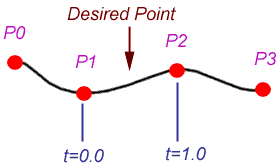
\includegraphics[width=0.4\textwidth]{images/curva-catmull.png}
			\caption{Ejemplo de curva de Catmull-Rom con 4 puntos que definen su forma. Obtenido de \cite{curves-catmull-rom-introduction}.}
				\label{fig:curva-catmull}
	\end{centering}
\end{figure}


El otro tipo de curva son las curvas de Bezier\cite{bezier-info}. Las curvas de Bezier se definen por 2 puntos, el origen y el extremo de la curva, y por al menos un punto más de control. Las curvas de Bezier con solo un punto de control se denominan curvas cuadráticas. Si tiene 2 puntos de control, se denomina curva de Bezier cúbica. Un ejemplo de curvas de Bezier cuadrática y cúbica se puede ver en las figuras \ref{fig:bezier-2} y \ref{fig:bezier-3}, respectivamente.


\begin{figure}[!ht]
	\begin{adjustwidth}{\oddsidemargin-1in}{\rightmargin}
	%	\centering
			\begin{subfigure}{\paperwidth}
				\centering
				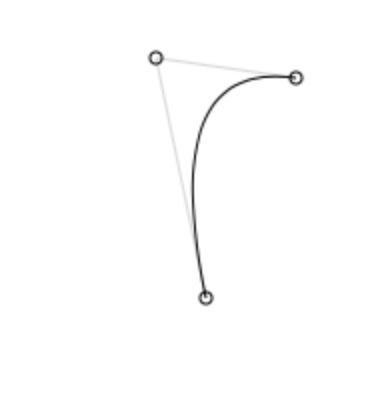
\includegraphics[scale=.5]{images/bezier-2.png}
	\caption{Ejemplo de curva de Bezier cuadrática. Obtenido de \url{http://pomax.github.io/bezierjs}.}				
				\label{fig:bezier-2}
			\end{subfigure}
			\begin{subfigure}{\paperwidth}
				\centering
				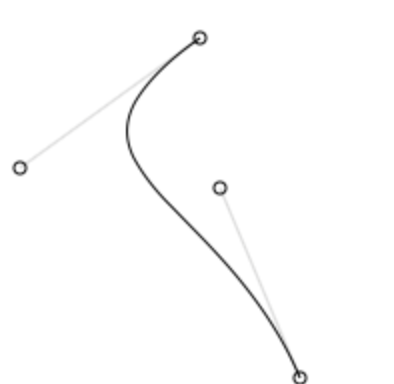
\includegraphics[scale=.5]{images/bezier-3.png}
	\caption{Ejemplo de curva de Bezier cúbica. Obtenido de \url{http://pomax.github.io/bezierjs}.}				
				\label{fig:bezier-3}
			\end{subfigure}
	\end{adjustwidth}
\end{figure}


Las curvas de bezier se definen en función de t, que se mueve en un intervalo de 0 a 1. Siendo \texttt{t=0} el inicio de la curva, \texttt{t=1} el final y \texttt{t=0.5} el punto intermedio. Una línea recta también puede ser representada mediante curvas de Bezier siempre que los puntos de control estén sobre la línea. No obstante, estas curvas tiene una limitación: no se puede representar un circunferencia con una (única) curva de Bezier. Esto es algo que no afecta a nuestro simulador.

Finalmente, para el modelado de líneas se ha decidido usar las curvas de Bezier, acompañado de la librería BezierJS\footnote{Página oficial del proyecto BezierJS (\url{http://pomax.github.io/bezierjs/}).} para Javascript. Esta librería ofrece una serie de funciones muy útiles para crear y manejar funciones. En el listado de código \ref{code:ejemplo-uso-bezier} se puede ver un ejemplo de las funciones más importantes de la librería. 

\begin{lstlisting}[language={Javascript},label={code:ejemplo-uso-bezier}, caption={Ejemplo de uso de las funciones de la librería BezierJS.}]
var curve = new Bezier (150,40 , 80,30 , 105,150);

var mid = curve.get(0.5);

var steps = 10;
var points = curve.getLUT(steps);
\end{lstlisting}

En la línea 1 del listado \ref{code:ejemplo-uso-bezier} se crea una curva cuadrática con los puntos \texttt{(150, 40)}, \texttt{(80, 30)} y \texttt{(105, 150)}. Concretamente, esta curva toma la forma de la curva de la figura \ref{fig:bezier-2}. El segundo punto es el punto de control. Una curva cubica se definiría de forma similar, pero pasando como argumento un punto de control más. 

En la línea 3 del listado \ref{code:ejemplo-uso-bezier} se obtiene el punto que está justo en la mitad de la curva. La función \texttt{getLUT()} devuelve un array de puntos equidistantes entre ellos dentro de la curva. El número de puntos es el valor de \texttt{steps} más 1.

La función \texttt{getLUT()} de la librería BezierJS será la clave para la detección de líneas en el simulador.


\subsubsection{Detectando curvas de Bezier}

Ahora que ya se ha aclarado que se usarán curvas de Bezier para representar las líneas en el simulador, solo queda saber la distancia de un punto (el sensor) al punto más cercano de la curva de Bezier. Este problema consiste en encontrar la proyección de un punto sobre una curva. Dicho problema ya ha sido estudiado anteriormente. Por ejemplo J. Ros en \cite{projection-point-bezier} estudia de manera matemática como resolver este problema. 

Teniendo esto en cuenta, ésta fue la primera aproximación al problema que se realizó. Los resultados no fueron buenos: el punto en la curva no era exacto y con un coste computacional alto.

En el segundo intento de resolución, se utilizaba la función \texttt{getLUT()} de BezierJS para partir la curva en muchas líneas rectas y crear un cuerpo en Box2D con muchas \texttt{fixtures}\footnote{Para crear la forma de línea recta en Box2D se utilizaba la clase \texttt{b2PolygonShape} estableciendo la forma con la función \texttt{SetAsEdge()} que recibe dos puntos y crea una línea entre ellos.}. De esta manera se conseguía formar una curva a partir de muchas líneas rectas. La detección de curvas, entonces, se realizaba igual que para los obstáculos (sección \ref{detectando-colisiones}).

Esto solucionaba el problema, pero la curva tenía una apariencia muy fina y se obtenía un coste alto al mantener una cantidad tan grande de cuerpos pequeños. Aunque se simplificara la curva con un valor de \texttt{step} suficientemente pequeño en la función \texttt{getLUT()}, no se solucionaba el problema de la línea fina.

La tercera aproximación al problema dio resultado. Era volver a proyectar el punto (sensor) sobre la curva, pero aproximando los puntos de ésta con la función \texttt{getLUT()}. De esta manera, se obtenía una cantidad razonable de puntos en la curva y se calculaba la distancia del sensor a cada uno de estos, resultando el problema en el cálculo de distancia entre dos puntos. Algo computacionalmente menos costoso que calcular la proyección de un punto sobre una curva. 

En el listado de código \ref{code:deteccion-bezier} se puede ver el código que detecta y notifica una \emph{colisión} con una línea. 

\begin{lstlisting}[language={Javascript},label={code:deteccion-bezier}, caption={Función que detecta líneas (curvas de Bezier).}]
function detectLineCollition(sensor) {
	var lines = Simulator.World.lines;
	var anysensed = false;

	// (...)

	var minDistance = Simulator.World.getDistanceCollitionLine();

	lines.forEach(function(curve) {
		var p = pointInBezier(curve, SensorPosition);
		// if any sensor collided, notify!
		var dist = distance(p, position);
		if (dist <= minDistance) {
			//notify the collision
			var message = {
				id: sensor.name,
				state: "begin"
			};
			sendMessage("sensor", message);
			anysensed = true;
			return;
		}

	});
	//if it detects no collitions, notify end collision
	if (!anysensed) {
		var message = {
			id: sensor.name,
			state: "end"
		};
		sendMessage("sensor", message);
	}
}
\end{lstlisting}

El valor de distancia mínima (variable \texttt{minDistance}) se define con el grosor de la línea más el radio del sensor.

La diferencia de esta última solución a la anterior es que en ningún momento se está creando la curva como objeto en Box2D. Por tanto, se ha modificado el prototipo de \texttt{World} para que almacene las líneas (variable \texttt{lines}). No obstante, siguen sin ser representadas con un objeto \texttt{Body} para ahorra coste y para facilitar el poder pintar distinto grosor de línea según convenga (por ejemplo, si se hace zoom en el circuito).

Con respecto al dibujo de las líneas, se explicará más adelante en la sección \ref{animando-robode}.


\subsection{Animando a Robode}
\label{animando-robode}


Para entender como se ha realizado la animación del simulador, primero es necesario conocer algunos conceptos de Javascript.

Javascript proporciona una serie de funciones para gestionar timers en la ejecución de un programa. Estos son:

\begin{itemize}
	\item \texttt{setTimeout(function, delay)}: Ejecuta la función \texttt{function} después de un tiempo especificado por \texttt{delay}. Devuelve un \texttt{id} que identifica al timer.
	\item \texttt{setInterval(function, delay)}: Ejecuta la función \texttt{function} de manera periódicamente cada vez que se cumple el \texttt{delay}. Devuelve un \texttt{id} que identifica al timer.
	\item \texttt{clearTimeout(id)} y \texttt{clearInterval(id)}: funciones que eliminan el timer asociado a ese \texttt{id}.
\end{itemize}

El uso normal que se haría en la aplicación (el simulador junto a Descubre) será ejecutar la función \texttt{setInterval(function, delay)} con un \texttt{delay} indicando cada cuanto tiempo se quiere ejecutar la función \texttt{function} (que en nuestro caso contendrá \texttt{World.Step()} y la actualización de los gráficos).

Por tanto, cada vez que se produzca un evento (por ejemplo, una interrupción de teclado o ratón), la ejecución de Javascript tratará dichos eventos. 

No obstante, Javascript tiene una limitación: implementa un sistema \emph{monohilo}. Esto implica que si hay una función que aún no ha terminado de ejecutarse cuando ocurre un timer o un evento, estos se verán retrasados hasta que dicha función acabe. Para más información, se puede consultar \cite{js-timers-works}, \cite{event-loop-js} y \cite{resig2013secrets}.

Además, hay que tener en cuenta el diseño de la aplicación (descrito en la sección \ref{sec:integracion-descubre}). Esta tendrá por una parte el \emph{sanbox} (clase \texttt{iJavaSandbox}) y por otra el simulador y la aplicación. El \emph{sandbox}  controlará la ejecución del programa escrito en iJava y enviará instrucciones al simulador (clase \texttt{Robode}). La aplicación atenderá a los eventos de teclado y ratón junto al simulador, que moverá el robot sobre el mundo.

A parte de todo esto, el Modelo de programación que se usará en el simulador (sección \ref{sec:modelo-programacion}) permitirá detener la recepción de instrucciones con la función \texttt{wait(n\_miliseg)} (API del simulador). Esto hará que la ejecución del \emph{sandbox} se bloquee un determinado tiempo. Pero esto no debe de ocurrir con el resto de la aplicación.


Se hace necesario separar ambas ejecuciones en dos hilos de ejecución diferentes. Un hilo ejecutaría la aplicación principal junto al simulador. El otro hilo ejecutaría el \texttt{Sandbox}, el cual podría detenerse y realizar una \emph{espera activa} cuando se ejecute la función \texttt{wait()}. De esta manera se consigue que el simulador se ejecute y sea controlado por el \emph{Sandbox} y las instrucciones que en éste se ejecutan.

Para conseguir esto, en Javascript existen los Web Workers\cite{web-worker-mdn}. Básicamente, un Web Worker permite ejecutar tareas en segundo plano separado del hilo principal. Es decir, se consigue un sistema \emph{multihilo} en Javascript. La comunicación del Web Worker con el resto de elementos se hace mediante mensajes, como los que se han visto anteriormente en los códigos \ref{code:begin-contact} o \ref{code:deteccion-bezier} y que vienen reflejados en el diagrama de clases de la figura \ref{fig:diagram-ijava-robode}.

Aún así, los Web Workers tienen sus limitaciones. La más importante es que no se puede interactuar con el DOM\footnote{El DOM (Document Object Model o Modelo de Objetos del Documento en español) es un API de programación para documentos de HTML. Parte fundamental de HTML y que contiene toda la información relacionada a la página web} de HTML. Esto hace que no se pueda dibujar en el \emph{canvas}. 

Entonces, la solución radica en convertir el \emph{Sandbox} en un Web Worker y que sea éste el que controle la ejecución del simulador mediante mensajes. De esta manera se consiguen separar el hilo de ejecución de la aplicación principal y el hilo que ejecutará las instrucciones de iJava.

En el hilo principal se ejecutará la función \texttt{setInterval()} con un valor de \texttt{delay} equivalente a 60 FPS (frames por segundo). Cada vez que se ejecute dicha función, se actualizarán las fuerzas del mundo, el movimiento del robot y se dibujará por pantalla el estado actual del mundo. En el código \ref{code:interval-function} se muestra la ejecución de la función \texttt{setInterval()}.

\begin{lstlisting}[language={Javascript},label={code:interval-function}, caption={Función \texttt{setInterval()} que se ejecutara 60 veces por segundo.}]
idInterval = window.setInterval(function() {
    Simulator.World.Step(
        1 / 60, //frame-rate
        10, //velocity iterations
        10 //position iterations
    );

    // Simulator.World.drawLines();
    Simulator.World.DrawDebugData();
    Simulator.World.ClearForces();

    updateMovement();

}, 1000 / 60);
\end{lstlisting}

En el hilo que ocupa el \emph{Sandbox}, se ejecutarán las instrucciones del programa y se atenderán los mensajes que lleguen desde el compilador pidiendo que se detenga o se reanude la ejecución (con un nuevo código), por ejemplo.


\subsubsection{Dibujando a robode}

Una vez que se ha aclarado como es la actualización del mundo, queda especificar como se dibuja el mismo.

Box2D provee un elemento para dibujar los objetos del mundo en el \emph{canvas} de HTML5, el objeto \texttt{b2DebugData}. Este pinta la forma de los cuerpos sobre el \emph{canvas} automáticamente. 

Pero como ya se ha mencionado anteriormente, las líneas no han sido representadas como elementos de Box2D, por tanto, se usarán las funciones nativas de \emph{canvas} para realizar esto. En el código \ref{code:dibujar-curvas} se puede ver el código que dibuja líneas implementado en el prototipo de la clase \texttt{World}.

\begin{lstlisting}[language={Javascript},label={code:dibujar-curvas}, caption={Función que dibuja las curvas de bezier en el \emph{canvas}.}]
Simulator.Env.b2World.prototype.drawLines = function() {
	var ctx = this.m_debugDraw.m_ctx;
	var scale = this.getWorldScale();
	ctx.save(); //save the current context
	ctx.lineWidth = this.lineThickness * scale;
	ctx.strokeStyle = "black";
	this.lines.forEach(function(l) {
		var points = l.points;
		ctx.beginPath();
		ctx.moveTo(points[0].x, points[0].y);
		if (points.length > 3) {
			ctx.bezierCurveTo(points[1].x, points[1].y, points[2].x, points[2].y, points[3].x, points[3].y);
		} else  {
			ctx.quadraticCurveTo(points[1].x, points[1].y, points[2].x, points[2].y);
		}
		ctx.stroke();
	});
	ctx.restore(); // restore the saved context
};
\end{lstlisting}

Para poder conseguir que esta función se ejecute, y ademas se pinten las líneas lo primero (para que esté en un plano inferior al robot y el resto de elementos) ha sido necesario modificar levemente la librería de Box2D. Esto era necesario porque Box2D limpia el \emph{canvas} antes de dibujar nada (borrando las líneas si se pintan antes de llamar a esta función y dibujando las líneas sobre el robot si se llama después). 

Esto se ha realizado añadiendo la llamada a la función \texttt{drawLines()} (si ésta está definida) en la implementación de la clase \texttt{b2DebugDraw}. La función \texttt{drawLines()} se ha definido como un prototipo del objeto \texttt{World}. El código \ref{code:redefinir-debug-draw} muestra esta modificación.

\begin{lstlisting}[language={Javascript},label={code:redefinir-debug-draw}, caption={Modificación de la librería de Box2D para poder dibujar de manera correcta las líneas.}]
// Draw function 
h.prototype.DrawDebugData = function(){ 
	   if(this.m_debugDraw!=null){
	   			//CLEAR THE CANVAS!
			   this.m_debugDraw.m_sprite.graphics.clear(); 
			   // my draw lines function (if it's defined)
			   if(this.drawLines){
					   this.drawLines();
			   }
			   // end re-defination
			   //(...)
		}
}
\end{lstlisting}

Adicionalmente se ha añadido un efecto de \emph{zoom}\footnote{Esto se ha realizado modificando la propiedad \emph{scale} del objeto \texttt{b2DebugDraw}.} que modifica el tamaño de todos los elementos, permitiendo crear circuitos más grandes y que se vea todo independientemente del tamaño del \emph{canvas}. Junto a esto, también se ha añadido un \emph{scroll} tanto vertical como horizontal por la pantalla para facilitar la visión del circuito cuando se realiza \emph{zoom}.
